%%%%%%%%%%%%%%%%%%%%%%%%%%%%%%%%%%%%%%%%%%%%%%
% Header
\documentclass[11pt]{report}
\usepackage[english]{babel}
\usepackage[utf8x]{inputenc}
\usepackage{amsmath}
\usepackage{hyperref}
\usepackage{graphicx}
\usepackage{fullpage}
\usepackage[normalem]{ulem}
\usepackage{listings}
\usepackage[lastexercise]{exercise}
\usepackage{enumitem}
\graphicspath{ {./img/} }

\begin{document}

\setlength{\parindent}{0cm}

\renewcommand{\ExerciseHeader}{\large\textbf{\ExerciseName~\ExerciseHeaderNB} - \textbf{\ExerciseTitle}\medskip}

\renewcommand{\ExePartHeader}{\medskip\textbf{\ExePartName\ExePartHeaderNB\ExePartHeaderTitle\medskip}}
%%%%%%%%%%%%%%%%%%%%%%%%%%%%%%%%%%%%%%%%%%%%%%
\title{Exercises -- Week 6: Importing Python Files}
\subsubsection*{EMAT10007 -- Introduction to Computer Programming}
\subsection*{\Large Exercises -- Week 6. Importing Python Files}



\subsection*{\Large 6.1 Packages and Modules}

\subsection*{Essential Questions}

\begin{Exercise}[title= Importing Python Modules]

\begin{verbatim}
                                geometry/
                                |
                                |---- __init__.py
                                |---- main.py
                                |---- volumes.py
\end{verbatim}



\Question{Create the file system shown above. Leave all .py files empty to begin with.}
\Question{In file volumes.py, write two functions, {\tt sphere} and {\tt cube}. Each function should take one input argument and return the volume of the shape in the name of the function. 
\Question{Edit the content of main.py so that when it is run, it prints the volume of a sphere of radius 3 m}.
\Question{Is there a way to achieve the same operation, using shorter code in main.py?}.
\Question{Add another file, areas.py within the `geometry' folder. In areas.py, write two functions, {\tt sphere} and {\tt cube}. Each function should take one input argument and return the surface area of the shape in the name of the function.}
\Question{Edit the content of main.py so that a variable {\tt A = 5 m} is created and the area and volume of a sphere of radius {\tt A} and a cube of side length {\tt A = 5 m} are printed.}
\end{Exercise}

\begin{Exercise}[title= Importing Python Modules from different sources]

\begin{verbatim}
                                building/
                                |
                                |---- __init__.py
                                |---- main.py
                                |---- funcs.py                        
                                |---- house.py

\end{verbatim}



\Question{Create the file system shown above. Leave all .py files empty to begin with.}
\Question{In file house.py, create three variables {\tt floor} = the floor number of the building as an integer, {\tt width} = the width of the building on this floor in metres as a float, {\tt length} = the length of the building on this floor in metres as a float, and assign them numerical values. }
\Question{In file funcs.py, create a function {\tt ceil} that returns the area of the ceiling using the height and width. }
\Question{Import all contents of house.py, and roof.py to main.py using {\tt *}. }
\Question{In file main.py, print the following when called, replacing {\tt <x>} and {\tt <y>} with the area of the value of variable {\tt floor} and the area calculated respectively:
\begin{verbatim}
The area of the ceiling on floor <x> is <y> m2
\end{verbatim}
}
\Question{In file main.py, calculate the height of the roof using {\tt width} as shown in Figure \ref{fig:roof}, where $\theta = \frac{\pi}{6}$ radians. Import all contents if the Python package {\tt math} to use trigonometric functions e.g. {\tt tan}. }
\Question{Look at the functions and variables in the {\tt math} package (https://docs.python.org/3/library/math.html) What potential namespace issues could arise in this program? Are any errors generated due to namespace issues when running your program? If so, how can you prevent them from happening? }
\Question{Instead of computing the roof height within the main file, create a function {\tt roof\_height} in funcs.py that returns this value, and call the function in main.py.  Notice how this effects use of functions and variables from {\tt math}. \\ If imported objects (e.g. {\tt math.pi}) are used to define a function, for example {\tt roof\_height}, then the module that the object belongs to (e.g. {\tt math}) must be imported in the file where the function is defined (e.g. funcs.py) rather than where it is called (e.g. main.py).}

\end{Exercise}

\begin{figure}[!h]
        \centering
        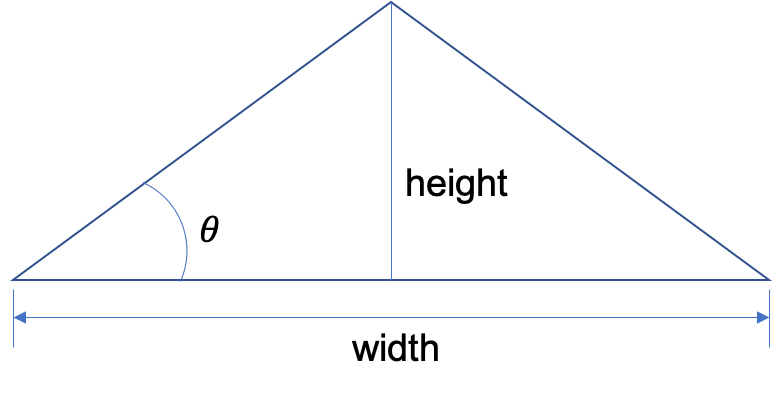
\includegraphics[height=5cm]{roof}
        \caption{Roof dimensions}
        \label{fig:roof}
\end{figure}

\subsection*{Advanced Questions}

\begin{enumerate}[label=(\Alph*)]
    
    \item Create your own Python module (.py file). For example, you could store some useful equations that you have learnt/used recently in another unit as Python functions. Or you could simply take some of the functions you wrote in Week 4 and practise assembling them as a Python module and importing them.  
    \item Practise different ways of calling variables, functions and classes from within main.py such as changing the namespace and importing individual functions and/or variables. 
    
\end{enumerate}

\pagebreak

\subsection*{\Large 6.2 Importing from other locations}

\subsection*{Essential Questions}

\begin{verbatim}

                        cubes/
                        |
                        |---- __init__.py
                        |---- cube.py
                        |---- shapes/
                                |
                                |---- main.py
                                |---- spheres/
                                        |
                                        |---- __init__.py
                                        |---- sphere.py
                                        
\end{verbatim}

\Question{Create the file system shown above. Leave all .py files empty to begin with.}

\begin{Exercise}[title= Importing from downstream locations]
    
    \Question{In file sphere.py, create a class {\tt Sphere} that takes one input argument, the radius. }
    \Question{Give the class two methods that return the surface area and volume of the sphere respectively.}
    \Question{Edit main.py to print the surface area of a sphere of radius 5 m. \\ {\bf Hint: } There are a number of ways to deal with the need for constants e.g. $\pi$ \\ The most reliable way to ensure a constant value is used is to import it from: 
    \begin{itemize}
        \item  an external package e.g. {\tt math} for well known constants like $\pi$
        \item a module created by you to store for program-specific constants - we'll try this out in the next question ...
    \end{itemize}
    }
    \Question{Create a sub-directory within `spheres' and a file within it, dimensions.py.}
    \Question{Create a variable within dimensions.py, {\tt radius} and give it a numerical value.} 
    \Question{Import the entire contents of dimensions.py to main.py and use {\tt radius} as the input argument to generate a {\tt Sphere} object.} 
    
\end{Exercise}

\begin{Exercise}[title=Importing from upstream locations]

    \Question{In file cube.py, create a class {\tt Cube} that takes one input argument, the side length with a default value of 1 m.}
    \Question{Give the class two methods that return the surface area and volume of the cube respectively.}
    \Question{Edit main.py to print the surface area of a cube with side length equal to the value of {\tt radius} in dimensions.py}

\end{Exercise}

\begin{Exercise}[title=Importing from upstream and downstream locations]\label{Ex:upstream_downstream}

    \Question{Create a new .py file upstream of main.py}\label{Q:new_file}
    \Question{Create a function in the file. }
    \Question{Call the function from within main.py }
    \Question{Create a new file downstream of main.py}
    \Question{Add some variables to the file}
    \Question{Print the variables within main.py }

\end{Exercise}

\subsection*{Advanced Questions}

\begin{enumerate}[label=(\Alph*)]
    
    \item Python files can be run as a module (imported file) or script (run as program, not imported). When the Python interpreter reads a Python file it sets some variables, then executes the code in the file. One of these variables is {\tt \_\_name\_\_}.\\ {\tt \_\_name\_\_} takes the value {\tt \_\_main\_\_} if the file is run as a script, and the value is the filename if the file is run as a module. The format shown below is widely used to allow a python file to be run as either a module or a script:
    
    \begin{verbatim}
    if __name__ == "__main__":
       print("Executed when file run directly")
    else:
       print("Executed when file imported")
    \end{verbatim}
    
    Edit the file you created in Exercise \ref{Ex:upstream_downstream}.\ref{Q:new_file} so that the function it contains is run (e.g. to test the function works) if the file is run directly, but not if the file is called as a module. 
    
    % \item \_\_init\_\_.py sometimes contains initialisation code that is run when a package or module is imported. For example, when a Python package is imported, python files within the directory can be automatically imported by adding a line of the form:
    
    % \begin{verbatim}
    % from . import <?>
    % \end{verbatim}
    
    % to \_\_init\_\_.py, where . signifies the current directory and <?> is the name of a python module in the current directory. 
    
    % Edit \_\_init\_\_.py in the spheres directory so that sphere.py is imported when sphere is imported. 
    
    
    
    
    
    

    \item Create another sub-directory within the `shapes' sub-directory and create your own python package. Create Python file(s) within the directory and practise calling them from within main.py
    
    
\end{enumerate}

\end{document}
